\documentclass[10pt,twocolumn]{article}
\usepackage[utf8]{inputenc}
\usepackage[T1]{fontenc}
\usepackage[margin=0.8in,columnsep=0.28in]{geometry}
\usepackage{graphicx}
\usepackage{booktabs}
\usepackage{amsmath}
\usepackage{url}

\graphicspath{{../figures/}}

\title{Solved, but How Late? A Measured Anytime Curve\\for a Local 4-bit Coding Agent under a Pooled Time Budget}
\author{Author names to be added}
\date{Draft v0.3, 14 October 2026}

\begin{document}

\maketitle
\begin{abstract}
\noindent
The competition studied here gives an agent a pooled 12 hours for all hidden tasks, so what matters is how much of its capability arrives early and what a per-task time cap costs. We study the Gemma~4 31B (4-bit) developer agent using 497 recorded runs on 71 verified tasks, a context-budget experiment (284 runs), and a new \emph{sequential} run of the same agent on all 71 tasks under the current harness (one task at a time, Kaggle 4$\times$L4, 13.3~s per tool call). That run resolves 45.1\% of tasks; 35\% are resolved within 6 minutes, which is the pool average for about 120 hidden tasks. Uncapped, the agent averages 5.5 minutes per task, leaving about 30 seconds for set-up; a 10-minute cap keeps 91\% of the score. Two thirds of tool calls go to runs that never resolve, yet issue text does not predict which tasks these are (leave-one-out AUC 0.51). Under a fixed total call budget one long attempt beats every split into retries, and edit-site size in read-window units predicts how many calls a fix takes (Spearman 0.51 [0.22, 0.74]).
\end{abstract}

\section{Introduction}
Small local coding agents are scored by the share of issues whose hidden tests pass, but a deployment bounds time. In this competition the rule is pooled: 12 hours for all tasks, including sandbox set-up and excluding patch validation, with optional per-task limits. The practical questions are therefore ``how early is the answer available?'' and ``what does a per-task cap cost?'', not only ``can the agent solve it?''. Public analyses of this competition study retrieval quality, harness failure modes, behaviour traces and leaderboard noise; we ask the budget question and answer it from measured runs.

\textbf{Contributions.} (1) A measured wall-clock anytime curve and a per-task-cap trade-off table for a sequential 71-task run, with task-clustered intervals. (2) Anytime curves in tool-call units from 497 recorded runs, which are invariant to concurrency. (3) A decomposition of where calls are spent and a fixed-budget retry analysis. (4) A test of which task properties explain lateness and solvability, including three negative results. (5) Open code on public run tables.

\section{Related Work}
\textbf{Trajectory behaviour.} Failed runs are longer and more variable than successful ones, and agents often reach the right files even when they fail \cite{majgaonkar}. Across 9,374 trajectories the underlying LLM matters more than the framework, and patch size alone does not explain difficulty \cite{mehtiyev}. File choice is too coarse to separate success from failure; function selection and completion behaviour localize the difference \cite{shu}.

\textbf{Difficulty.} Static task features predict difficulty before any run (AUC 0.863), with patch fragmentation and repository scale the largest drivers \cite{alhaque}. Our fix-size result agrees, and we add a time-to-patch axis.

\textbf{Harness, context and localization.} Context management mostly acts by preventing overflow and matters most under tight budgets \cite{fan}. Graph-guided localization is studied in LocAgent \cite{locagent}.

\textbf{Early termination.} EET \cite{eet} cuts agent cost by 19--55\% on SWE-bench Verified by stopping unproductive iterations using experience from earlier runs. It targets cost at fixed success; we measure how much score is available by a given time and whether any deployable signal can route time.

\textbf{Within this competition,} public notebooks audit retrieval, document an output-cap/context interaction and a coupled-timeout trap, and analyse leaderboard noise. We differ in measuring time-to-resolution directly.

\section{Setting and Data}
\textbf{Agent and harness.} The competition's model (Gemma~4 31B, QAT W4A16), nine tools including three code-graph tools, vLLM with a 32,768-token window (16,384-token input ceiling), event compaction, and per-task budgets of 40 tool calls, 30 minutes and 100 turns in all runs we report.

\textbf{Official budget.} 12 hours for all tasks. The test set has ``about 120 tasks'', evenly split between public and private splits and curated from private repositories (competition data page): about 6.0 minutes per task on average.

\textbf{Recorded runs.} Public per-run tables of an earlier study (Apache-2.0): 71 verifiable tasks (rich 42, fastapi 29), $7\times71=497$ observational runs and $4\times71=284$ runs varying input budget and compaction threshold. Those sessions ran 12--14 agents concurrently on one server, so their durations are 2.8--3.4$\times$ inflated and are not used as time.

\textbf{New sequential run.} The competition's starter harness with current settings (compaction interval 15, thinking budget), a single-agent configuration and the recorded study's budgets, on Kaggle 4$\times$L4, one task at a time, all 71 tasks, one run each, in two kernels of 36 and 35 tasks. A separate 8-task calibration (31B and 12B) preceded it.

\section{Methods}
\textbf{Units.} Tool-call ordinal for recorded runs; wall-clock minutes of agent time for the new run (includes about 3--4~s of subprocess sandbox set-up and verification; excludes model load).

\textbf{Semantics.} \emph{Completed}: resolved and finished by $k$ calls (or $t$ minutes), a lower bound. \emph{In place}: the final patch already existed in the working tree by call $k$, closer to the harness's patch recovery; shell-made edits are invisible to it.

\textbf{Cap trade-off.} For a per-task cap $c$, the resolved share is the share resolved with duration $\le c$, mean time per task is $\mathrm{mean}(\min(\text{duration},c))$, and tasks fitting in 12 hours is $720/\text{mean minutes}$ (set-up time excluded).

\textbf{Retries.} A total budget $B$ split into $k$ equal attempts, estimated per task from recorded runs under an independence assumption.

\textbf{Uncertainty.} Task-clustered bootstrap, 2,000 replicates; intervals are 95\%.

\textbf{Driver screen.} 24 exploratory feature--outcome Spearman correlations; the surviving result is checked within repository, in an independent session and under partial control.

\textbf{Analysis status.} The new-run analyses (resolved share, call curve, latency, overflow) were stated before the results were seen. The wall-clock curve and cap table were added afterwards and are flagged as post hoc.

\section{Results}

\subsection{The measured wall-clock curve}
The sequential run resolves 45.1\% [33.8, 56.3] of tasks, against 39.2\% [29.0, 49.5] for the recorded runs on the same tasks (paired difference $+5.8$ points [0.8, 11.1]). We do not attribute the difference to the harness changes. A replicate of one half of the tasks (36 tasks, same model, harness and budgets, run on a separate kernel) resolves 41.7\% against 44.4\% in the first run on those tasks; 33 of 36 outcomes agree (3 flips, 2 in one direction and 1 in the other; paired difference $-2.8$ points [$-11.1$, $5.6$]). Against recorded runs on the same 36 tasks (35.3\%) the two runs differ by $+9.1$ [2.0, 17.9] and $+6.3$ [$-2.4$, 15.1] points; their mean is $+7.7$ [1.2, 15.1]. The replicate bounds run-to-run noise at about three tasks in 36 and supports a modest gain over the recorded runs, but with 36 tasks the interval still includes zero for one run, so we call it suggestive. Pooled latency in the replicate is 13.5 s per tool call [11.2, 16.2] (first run 14.8 on the same tasks). Median task time is 4.1 minutes (p90 10.2, maximum 20.3; no run reached 30). Pooled latency is 13.3~s per tool call [11.5, 15.3] (task median 11.1; 8-task calibration 15.6) against 44~s in the concurrent sessions. Table~\ref{tab:time} and Fig.~\ref{fig:wall} show the curve.

\begin{table}[t]
\centering
\caption{Resolved share by wall-clock time, sequential run (71 tasks).}
\label{tab:time}
\small
\begin{tabular}{lccccc}
\toprule
Minutes & 3 & 5 & 6 & 10 & 15 \\
\midrule
Resolved & 18\% & 32\% & 35\% & 41\% & 44\% \\
95\% interval & --- & [23, 44] & [24, 46] & --- & --- \\
Share of final & 41\% & 72\% & 78\% & 91\% & 97\% \\
\bottomrule
\end{tabular}
\end{table}

\begin{figure*}[t]
\centering
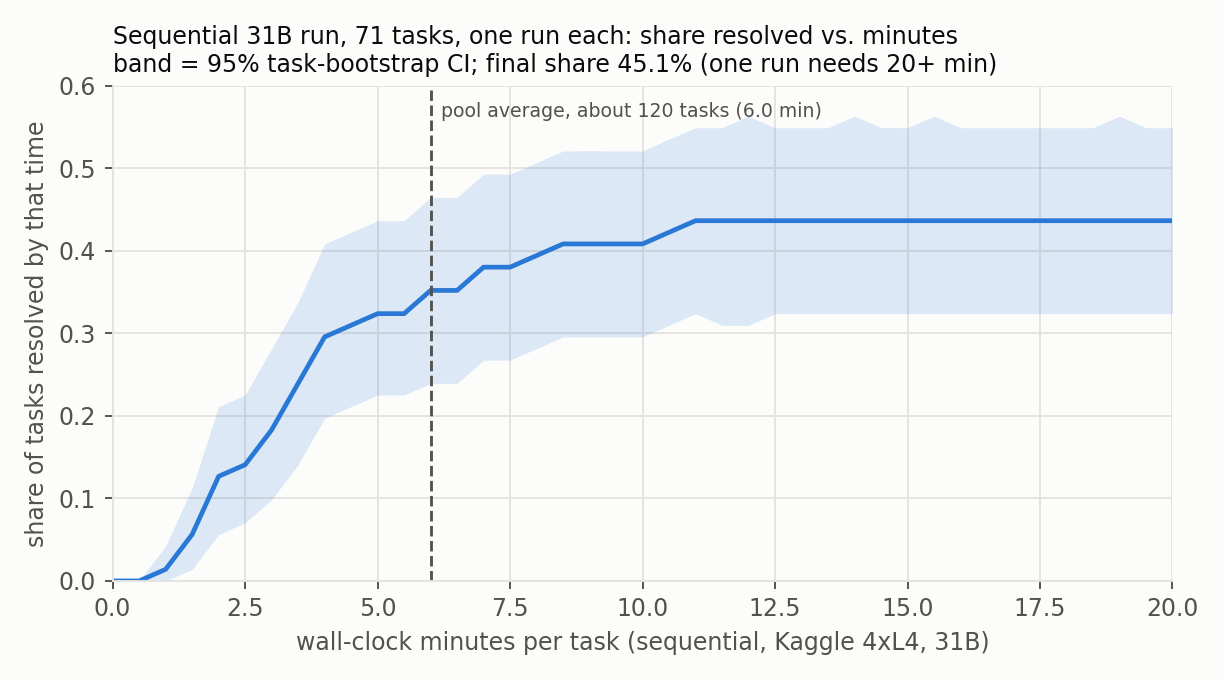
\includegraphics[width=0.72\textwidth]{fig1_wall_clock_curve.png}
\caption{Share of tasks resolved against wall-clock minutes for the sequential 31B run (71 tasks, one run each, Kaggle 4$\times$L4). Shaded band: 95\% task-bootstrap interval. Dashed line: 6.0 minutes, the pool average for about 120 tasks.}
\label{fig:wall}
\end{figure*}

\subsection{What a per-task cap costs}
Because the budget is pooled, a cap can be set without the average changing much (Table~\ref{tab:cap}). With about 120 tasks the pool is 6.0 minutes per task. Uncapped, the agent's mean of 5.5 minutes uses 11.0 of the 12 hours and leaves 29 seconds per task for sandbox set-up, which counts against the pool and which we could not measure. A 10-minute cap keeps 91\% of the score and leaves 57 seconds per task; a 6-minute cap keeps 78\% and leaves 105 seconds. The cap is therefore a safety margin against set-up time and slower hidden tasks, not a gain in score.

\begin{table}[t]
\centering
\caption{Per-task cap trade-off, sequential run (post hoc). ``Resolved'' means resolved with duration $\le$ cap (a lower bound). Slack is seconds per task left over at 120 tasks.}
\label{tab:cap}
\small
\begin{tabular}{rrrrr}
\toprule
Cap (min) & Resolved & Mean (min) & Tasks/12~h & Slack (s) \\
\midrule
4 & 29.6\% & 3.4 & 212 & 156 \\
6 & 35.2\% & 4.3 & 169 & 105 \\
10 & 40.8\% & 5.0 & 143 & 57 \\
15 & 43.7\% & 5.4 & 134 & 38 \\
none (30) & 45.1\% & 5.5 & 131 & 29 \\
\bottomrule
\end{tabular}
\end{table}

\subsection{Anytime curve in tool calls}
In recorded runs, in-place resolution is 8.2\% at 10 calls, 17.5\% at 15, 24.3\% at 20, 31.4\% at 30 and 38.8\% at 40; 45\% of the final score exists by 15 calls (Fig.~\ref{fig:calls}). The new run's completed curve is similar (14.1\% at 15, 23.9\% at 20, 31.0\% at 30, 45.1\% at 40). Mapping calls to minutes with the pooled latency (27 calls at 6 minutes) gives about 30\% in place, against 35\% measured directly, because resolved runs use fewer and cheaper calls than unresolved ones.

\begin{figure*}[t]
\centering
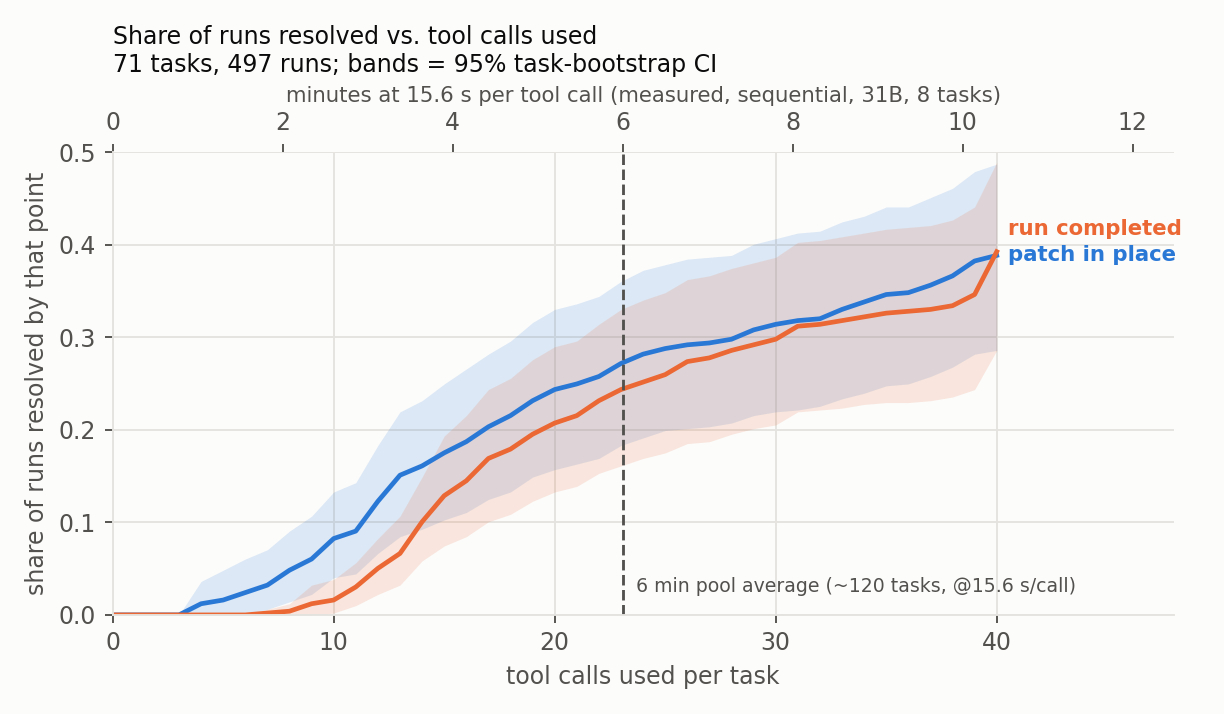
\includegraphics[width=0.72\textwidth]{fig2_call_curve.png}
\caption{Recorded runs (71 tasks, 497 runs): share resolved against tool calls used, under two semantics. Bands: 95\% task-bootstrap intervals. Top axis converts calls to minutes at the 8-task calibration latency of 15.6~s per call; the dashed line is 6 minutes at that latency.}
\label{fig:calls}
\end{figure*}

\subsection{Where the calls go}
In recorded runs 12\% of calls are exploration before the first edit, 18\% editing and 5\% verification after the final edit; unresolved runs consume 22\% (gave up), 21\% (call budget), 15\% (timeout) and 8\% (context overflow) (Fig.~\ref{fig:where}). Thirty-two of 71 tasks are never solved in seven runs and absorb 49\% of calls; an oracle cutting them at 10 calls would free 32\%. A deployable predictor from issue text has leave-one-out AUC 0.51 [0.38, 0.64], so this bound is not reachable. In the new run the same split holds: 100\% of always-solved, 64\% of mixed and 3\% of never-solved tasks were resolved.

\begin{figure*}[t]
\centering
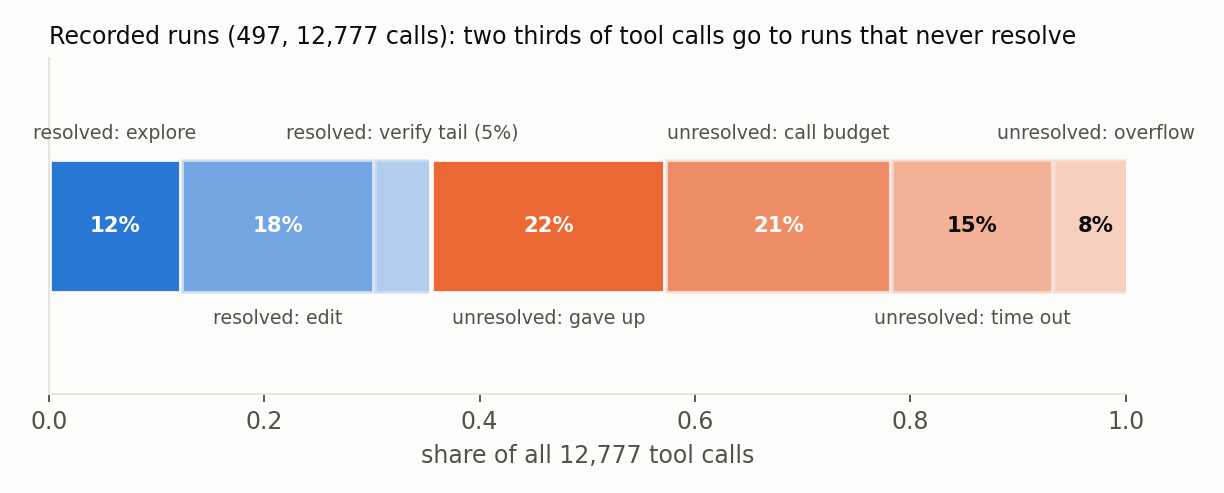
\includegraphics[width=0.72\textwidth]{fig3_where_calls_go.png}
\caption{Recorded runs: share of all 12,777 tool calls by outcome and phase.}
\label{fig:where}
\end{figure*}

\subsection{Retries do not help under a fixed budget}
With total budgets of 20 / 30 / 40 calls, one attempt resolves 24.3\% / 31.4\% / 38.8\% against 11.7\% / 22.3\% / 29.9\% for two attempts (Fig.~\ref{fig:retries}). Successful runs need about 17 calls to the final patch, so short attempts rarely finish.

\begin{figure*}[t]
\centering
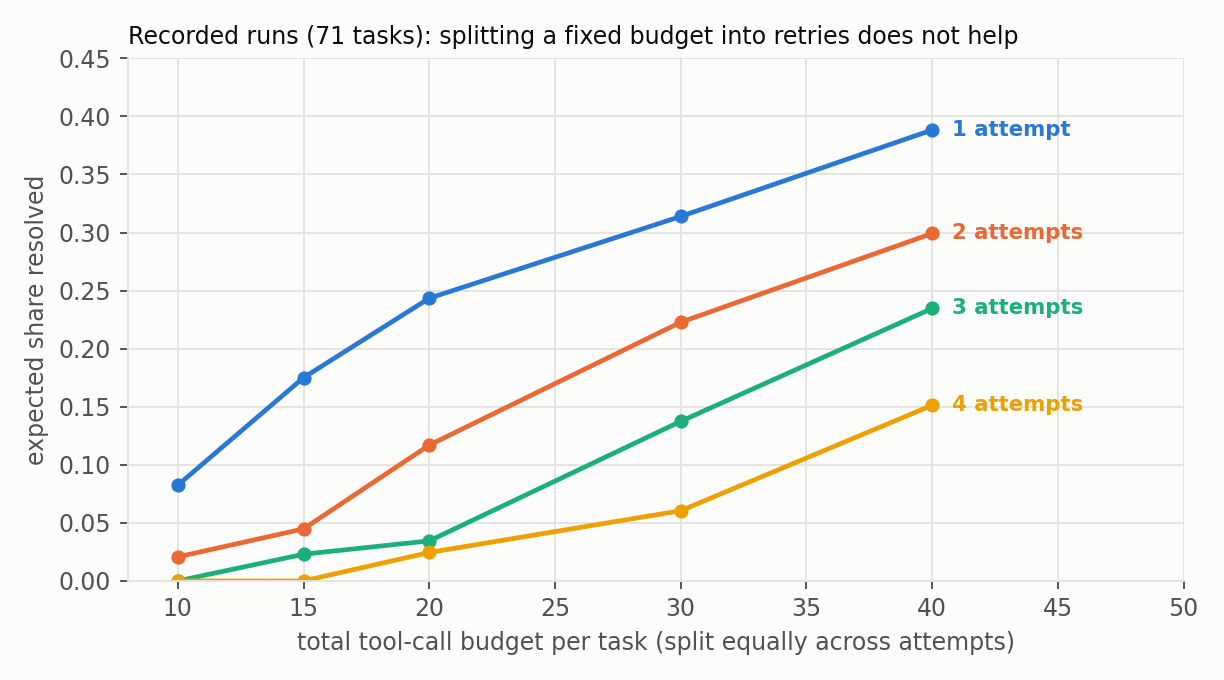
\includegraphics[width=0.72\textwidth]{fig4_retries.png}
\caption{Expected share resolved when a fixed total call budget is split into $k$ equal independent attempts (recorded runs, patch-in-place semantics).}
\label{fig:retries}
\end{figure*}

\subsection{What explains lateness}
The number of 150-line read windows needed to cover the edited files predicts calls-to-patch among solved tasks (Fig.~\ref{fig:window}, Table~\ref{tab:rho}). Patch size explains \emph{whether} a task is solved ($\rho=-0.53$ [$-0.69$, $-0.35$]) but not how many calls it takes (0.14 [$-0.20$, 0.47]).

\begin{table}[t]
\centering
\caption{Read windows against median calls-to-patch among solved tasks: Spearman $\rho$ with 95\% task-bootstrap intervals.}
\label{tab:rho}
\small
\begin{tabular}{lrl}
\toprule
Check & $n$ & $\rho$ \\
\midrule
All observational runs & 39 & 0.51 [0.22, 0.74] \\
Context-experiment run & 35 & 0.57 [0.27, 0.80] \\
fastapi only & 16 & 0.57 [0.08, 0.84] \\
rich only & 23 & 0.35 [$-0.10$, 0.71] \\
Partial (controls) & 39 & 0.51 \\
\bottomrule
\end{tabular}
\end{table}

\begin{figure*}[t]
\centering
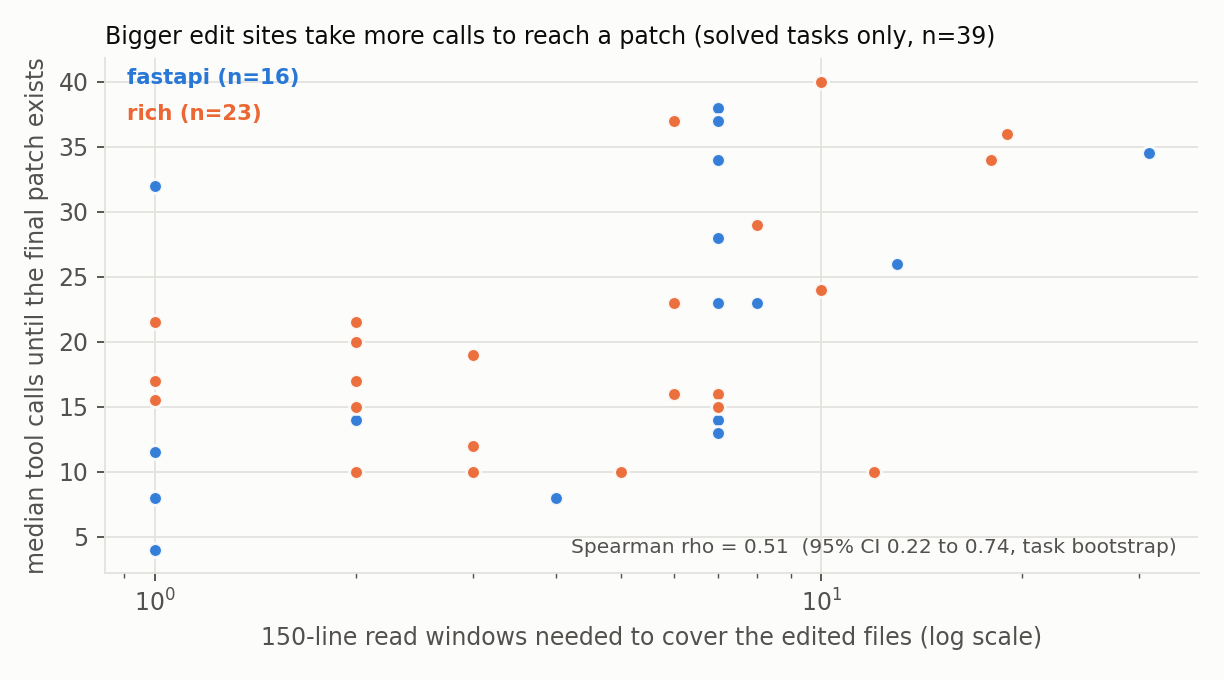
\includegraphics[width=0.72\textwidth]{fig5_window_cost.png}
\caption{Harness read-window cost of the edit site against median tool calls until the final patch exists (solved tasks only, $n=39$).}
\label{fig:window}
\end{figure*}

\subsection{Negative results}
Window cost does not predict context overflow ($\rho=-0.16$ [$-0.38$, 0.07]). Prompt-size trajectories in the first eight calls do not predict overflow (AUC 0.50--0.58). Issue text does not predict solvability (AUC 0.51). Raising the input budget solved more tasks (23/22 to 30 of 71) without making solved tasks faster (median final-patch call 13--16).

\subsection{Model size (indicative, 8 tasks)}
The 12B model decoded 1.8$\times$ faster (52 vs 29 tokens/s) but wrote longer reasoning, so time per tool call was similar (12.9 vs 15.6~s). On the three tasks both solved it needed 85 tool calls and 1,380~s against 47 calls and 488~s, and four of eight 12B runs overflowed the input ceiling versus none for 31B. Faster decoding was not faster solving here.

\section{Discussion}
For a pooled, latency-bounded evaluation, a fixed agent's score depends on how the budget is distributed, not only on per-call speed. First, most of the score arrives early: 35\% of tasks by 6 minutes of a 45\% total, so a moderate cap is cheap. Second, retries do not help at small budgets, so spare time is better spent on one longer attempt than on restarts. Third, solvability and lateness are different problems: patch complexity governs \emph{whether} a task is solved, edit-site size governs \emph{how late}. The absence of a deployable difficulty signal argues against routing time by issue text, and cheaper localization (fewer windows read before the first edit) is the lever for lateness.

\section{Limitations}
\begin{enumerate}
\item One run per task in the full sequential run; a replicate of 36 tasks shows 3 outcome flips, so the $+5.8$-point difference to recorded runs is suggestive, not established.
\item 71 tasks from two repositories, a selective sample (58 public tasks fail the reference patch in the local environment); hidden test repositories are private.
\item Latency is measured in a subprocess sandbox and excludes model load; subprocess set-up was measured at a median of 3.6~s per task (included in all durations), but the official containers' set-up is unmeasured and counts against the 12 hours.
\item The test set is ``about 120'' tasks from private repositories, so its time distribution may differ from our 71 public tasks. We therefore report the cap table rather than a single allowance.
\item The recorded sessions predate documented harness changes (compaction interval, thinking budget, three additional permitted models); the new run uses the current starter harness.
\item One agent configuration; participants may change prompts, tools and budgets. The model-size note is $n=8$ and indicative only.
\item Exploratory analysis with a 24-comparison screen; the replication reuses the same tasks. ``In place'' cannot see shell-made edits; retry independence is assumed.
\item The recorded-run dataset's page lists no licence; its repository includes an Apache-2.0 LICENSE file and README statement, which is what we rely on.
\end{enumerate}

\section{Reproducibility}
All numbers derive from public per-run tables, competition files available to participants, and the sequential-run result table. Code rebuilds tables, curves, figures and result files offline in minutes on a laptop (\texttt{reproduce.sh}); the Kaggle notebook builder is included. Per-task labels and task text are not redistributed (competition rules). Recorded-run numbers reproduce from public tables; the sequential run is released as aggregates.

\begin{thebibliography}{9}
\small
\bibitem{majgaonkar} O. Majgaonkar, Z. Fei, X. Li, F. Sarro and H. Ye, ``Understanding code agent behaviour: An empirical study of success and failure trajectories,'' arXiv:2511.00197, 2025.
\bibitem{mehtiyev} T. Mehtiyev and W. Assun\c{c}\~ao, ``Beyond resolution rates: Behavioral drivers of coding agent success and failure,'' arXiv:2604.02547, 2026.
\bibitem{shu} R. Shu, C. Y. Chong, X. Zhou, Y. Peng, Z. Wu, X. Han \emph{et al.}, ``What resolve rate hides: Trajectory structure diagnostics for coding agents,'' arXiv:2607.06184, 2026.
\bibitem{alhaque} E. Al-Haque and B. Johnson, ``What makes software issue resolution tasks difficult for agents?'' in \emph{Proc. ESEM}, 2026; arXiv:2608.18280.
\bibitem{fan} R.-Z. Fan, Z. Zhang, S. Ma, Y. Hu, S. Wang, K. Song \emph{et al.}, ``An empirical study of harness design for coding agents,'' arXiv:2609.20804, 2026.
\bibitem{locagent} Z. Chen, X. Tang, G. Deng, F. Wu, J. Wu, Z. Jiang \emph{et al.}, ``LocAgent: Graph-guided LLM agents for code localization,'' in \emph{Proc. ACL}, 2025; arXiv:2503.09089.
\bibitem{eet} Y. Guo, Y. Xiao, J. M. Zhang, M. Harman, Y. Lou, Y. Liu \emph{et al.}, ``EET: Experience-driven early termination for cost-efficient software engineering agents,'' in \emph{Findings of ACL}, 2026; arXiv:2601.05777.
\end{thebibliography}
\end{document}
